%!TEX root = ../../main.tex
\section{Results}
\label{sec:Results - Zero-dose extrapolation}
The extrapolation algorithm presented in section \ref{sec:Extrapolation routine} has been written in the Matlab programming language.
Intensity data from a single insulin crystal (crystal ID 0259) were collected as described in section \ref{sub:Data Collection and Dose Calculation} and processed as outlined in section \ref{sec:Extracting Intensities and Doses}.
The first 5000 reflections from five 90$^{\circ}$ degree datasets were used to perform zero-dose extrapolation.
The average DWD and scaled relative intensity values for each dataset are given in Table \ref{tab:Average DWD and Relative Intensity}.
The doses here represent the average doses in the dose shells used in the probabilistic extrapolation.
\begin{table}[ht!]
	\caption[Average DWD and scaled relative intensity values.]{Average DWD and scaled relative intensity values. The scaling value, $k$, was 1.0888}
	\centering
	\begin{tabular}{p{3.2cm} | p{3.75cm} | p{3.3cm}}
		Dataset Number    & Average DWD (MGy)     & Relative Intensity \\
		\hline
		1                 & 0.91                  & 0.9184 \\
		2                 & 2.50                  & 0.7812 \\
		3                 & 4.09                  & 0.6533 \\
        4                 & 5.68                  & 0.5252 \\
        5                 & 7.28                  & 0.4286 \\
	\end{tabular}
	\label{tab:Average DWD and Relative Intensity}
\end{table}
The 25,000 rows of data from the \textit{HKL} list in the MTZ files resulted in 1255 unique reflections on which the extrapolation as described in section \ref{sec:Extrapolation routine} was performed.
The minimum number of observations to perform the extrapolation was set at 8, and the threshold correlation coefficient was set at 0.5.
These values were chosen by inspecting a subset of extrapolated curves to determine which values generally resulted in curves that gave visually sufficient fits to the data.
The values chosen are quite conservative so it is expected that values which would result in a higher number of reflections extrapolated via the regression method (i.e. lower number of observations and lower correlation coefficient) may lead to better overall extrapolated values.
If the natural logarithm of any intensity values were over 14 then regression based extrapolation was not performed on the reflection.
This value was chosen because the plot of the data (Figure~\ref{fig:Before extrapolation all observations - Extrapolation method}) visually show that values beyond 14 are highly unlikely.
With those criteria, the conventional regression analysis was only performed on 748 (59.60\%) of the 1255 unique reflections.
The rejection list was as follows:
\begin{itemize}
    \item 43 (3.43\%) reflections were rejected because there were less than 8 observations.
    \item 375 (29.88\%) reflections were rejected because the first 8 intensity observations were too small.
    \item 89 (7.09\%) reflections were rejected because the correlation coefficient was below 0.5.
\end{itemize}
The assessment criteria for the regression fits are shown in Table~\ref{tab:R_fit and R_zero values}.
Both $R_{fit} < R^{thresh}_{fit}$ and $R_{zero} < R^{thresh}_{zero}$, suggesting that the regression fits and zero-dose extrapolated intensity values are sensible.
\begin{table}[ht!]
	\caption[Regression fit quality indicators.]{Regression fit quality indicators.}
	\centering
	\begin{tabular}{p{1.5cm} | p{1.5cm} | p{1.5cm} | p{1.5cm}}
		$R_{fit}$     & $R^{thresh}_{fit}$    & $R_{zero}$   & $R^{thresh}_{zero}$  \\
		\hline
		0.1359        & 3.7561                & 0.0977       & 0.1799        \\
	\end{tabular}
	\label{tab:R_fit and R_zero values}
\end{table}
Fits from two of the successfully extrapolated reflections are shown in Figure~\ref{fig:Successful zero-dose extrapolations}.
It is apparent from these two reflections that the behaviour of the intensities is very different.
Despite the general decrease in the average reflection intensities throughout the experiment, some reflection intensities increase before they start to decay (Figure~\ref{fig:Non-monotonic extrapolation}).
\begin{figure}
        \centering
        \begin{subfigure}[b]{0.9\textwidth}
                \centering
                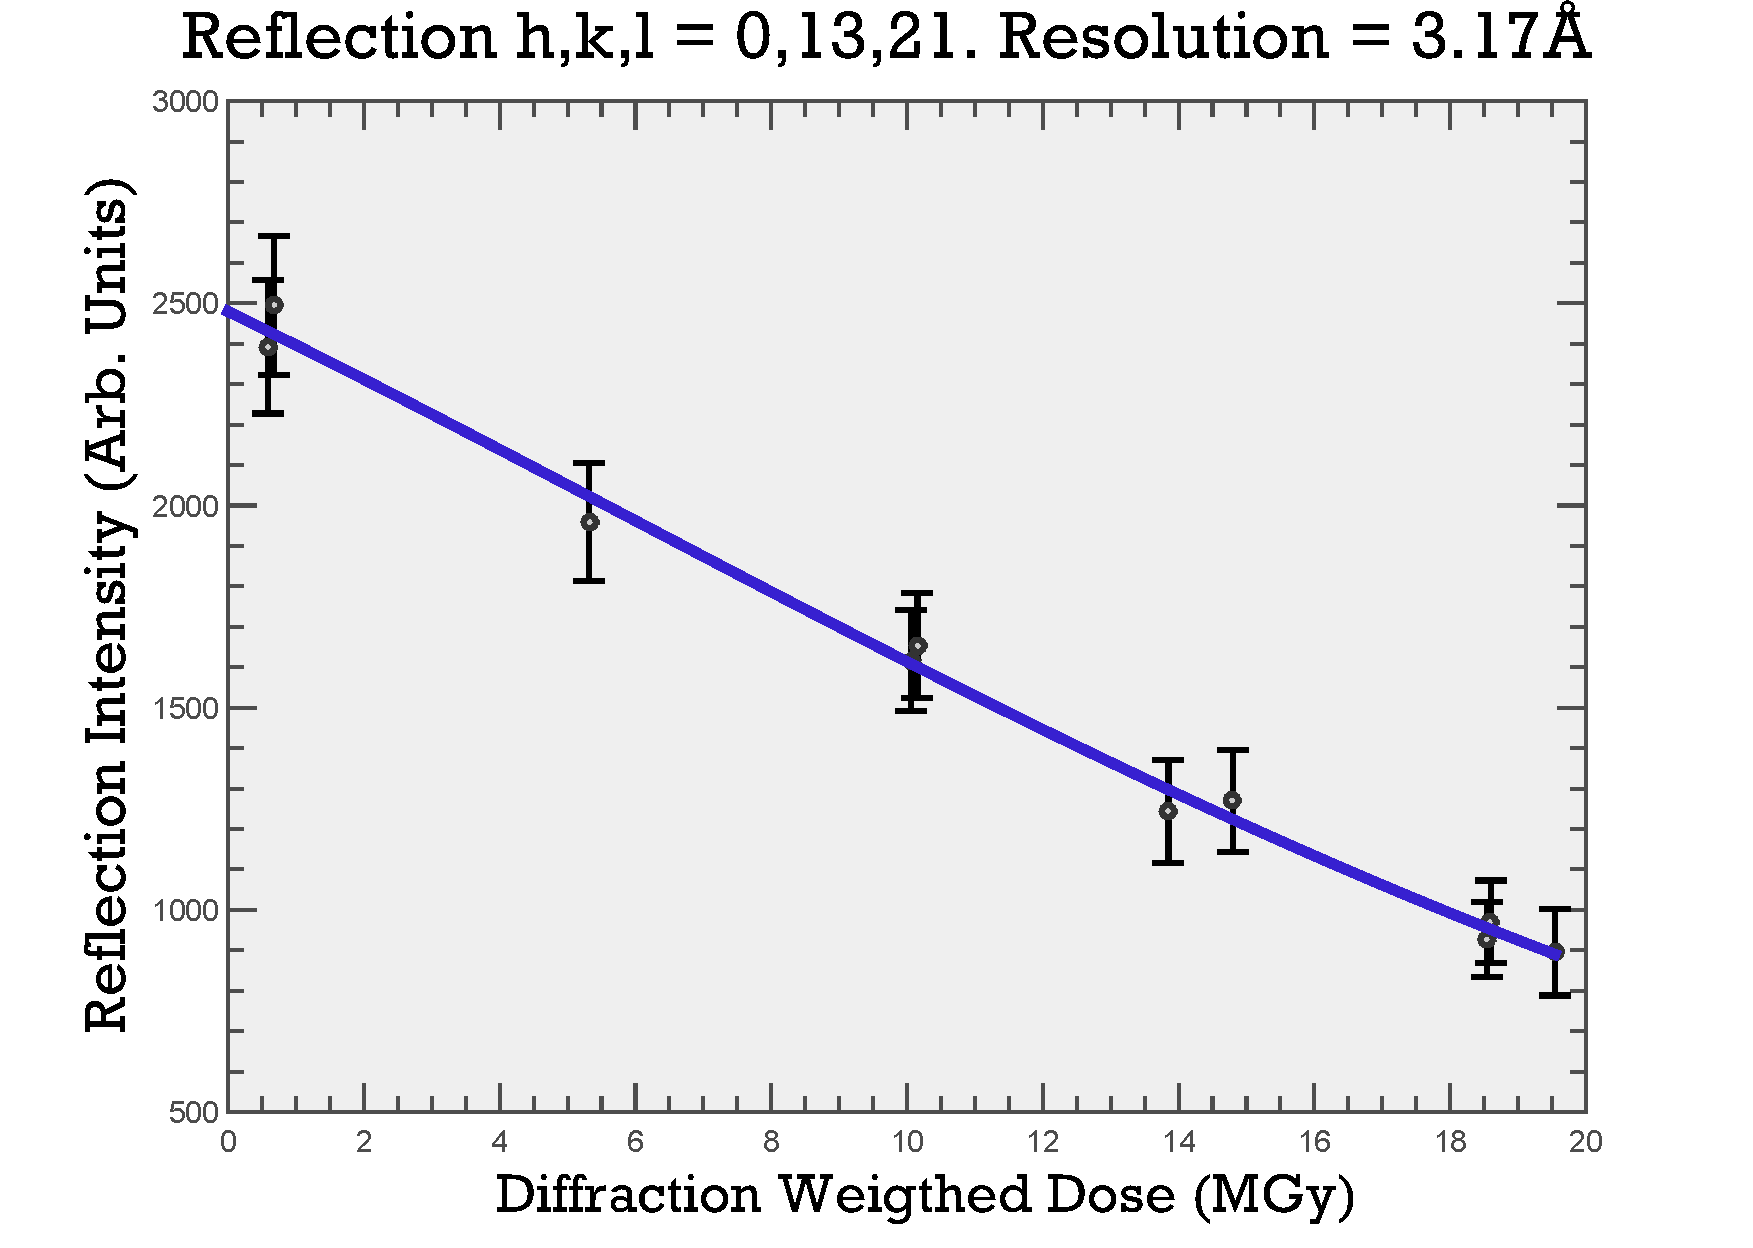
\includegraphics[width=1.0\textwidth]{figures/zde/Reflection-0,13,21.pdf}
                \caption{}
                \label{fig:monotonic extrapolation}
        \end{subfigure}
				\\
        \begin{subfigure}[b]{0.9\textwidth}
                \centering
                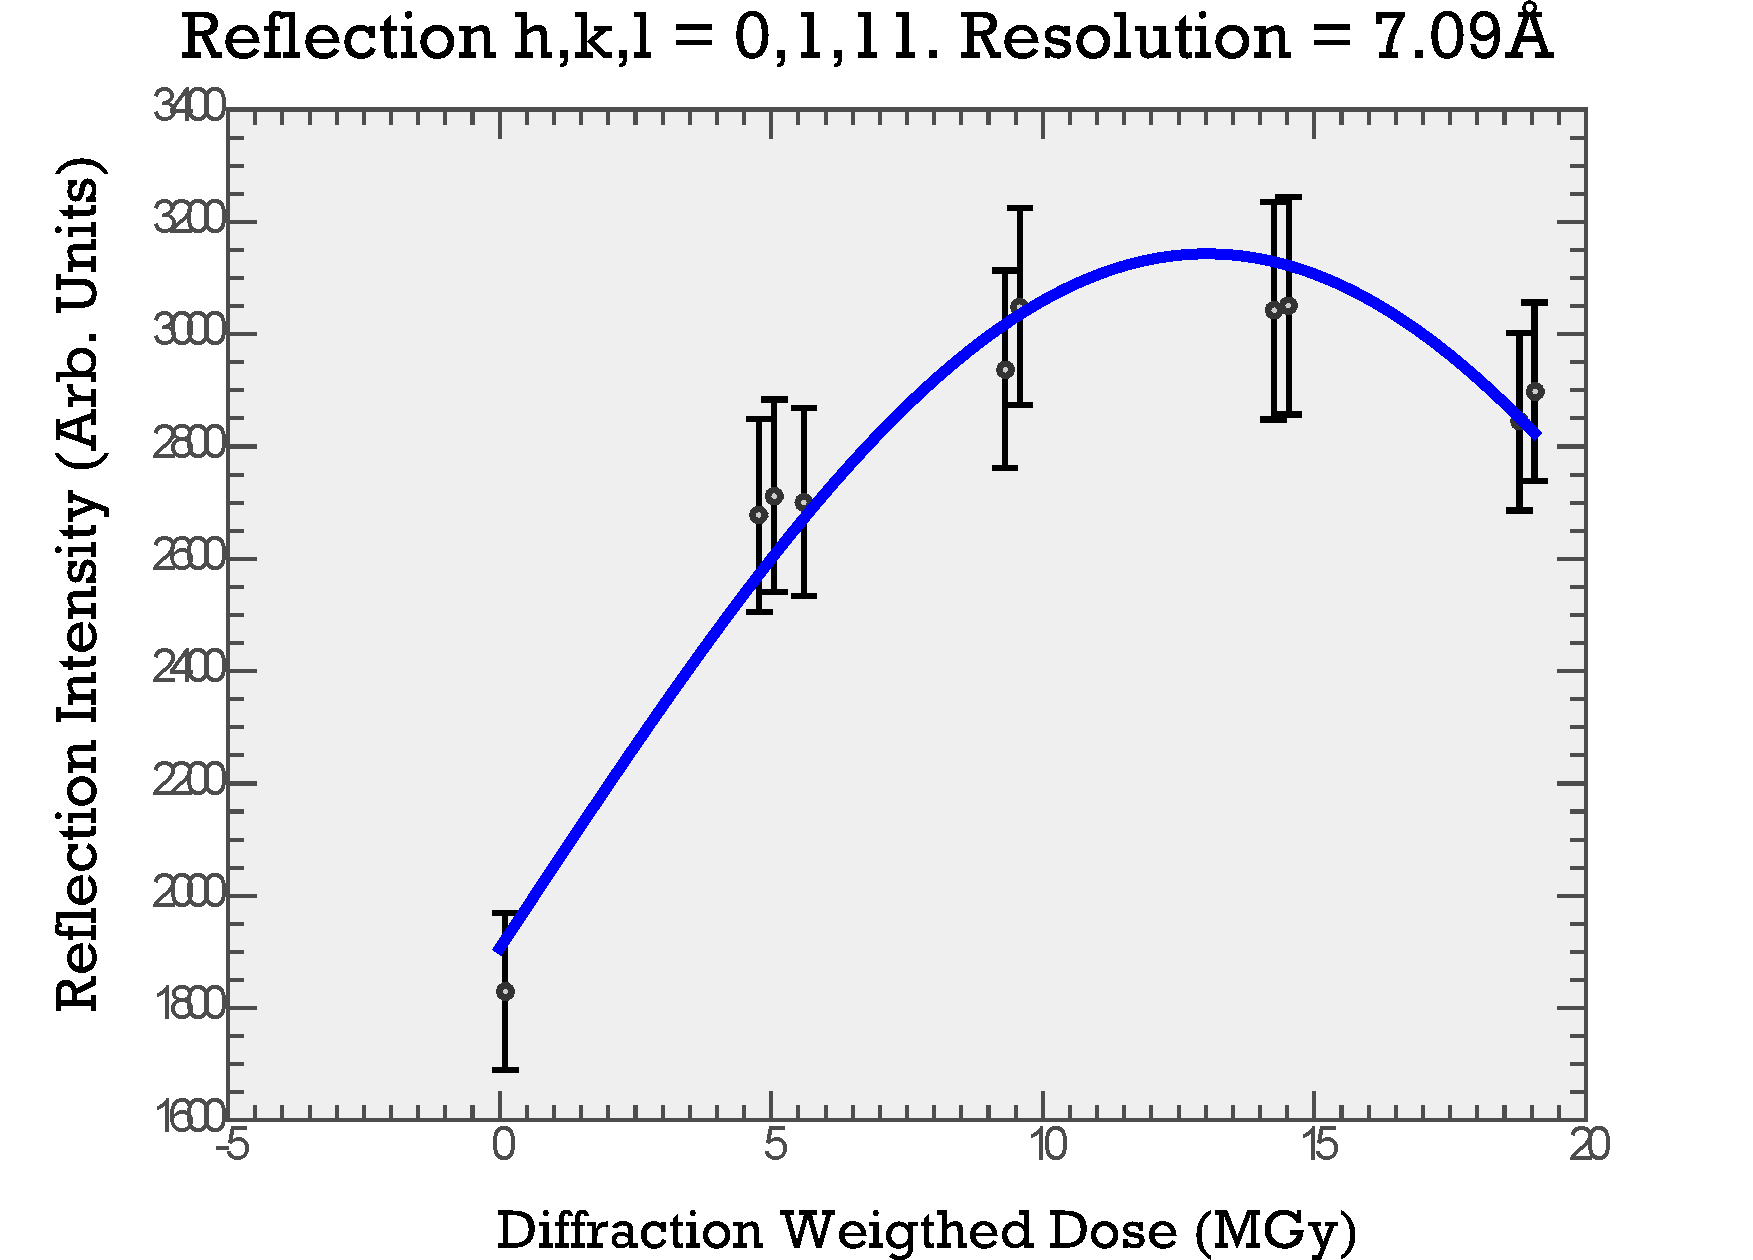
\includegraphics[width=1.0\textwidth]{figures/zde/Reflection-0,1,11.pdf}
                \caption{}
                \label{fig:Non-monotonic extrapolation}
        \end{subfigure}
        \caption[Regression fits that satisfied the regression criteria.]{Regression fits that satisfied the regression criteria outlined in section \ref{sub:Regression extrapolation} for two centric reflections.
		(a) The intensity of this reflection decreases linearly and monotonically.
		(b) The intensity increases before it starts to decrease.
		These are examples of the variety and non-linearity in the behaviour of individual reflection intensities.}
        \label{fig:Successful zero-dose extrapolations}
\end{figure}

A total 507 of the 1255 reflections (40.40\%) were rejected for the regression fits and were thus extrapolated using the probabilistic approach.
The calculated distributions for 2 centric reflections are shown in Figure~\ref{fig:Probabilistic distributions - Extrapolation method}.
The extrapolated intensities for negative reflection intensities are made positive because the Wilson distribution has a zero probability value for negative reflection intensities.
The intensity values for weak reflections are significantly affected by the prior distribution.
This is evidenced by the fact that the posterior distribution resembles the prior distribution for weak reflections (Figure~\ref{fig:Weak negative reflection intensity - Extrapolation method}).
In contrast, strong reflections are almost unaffected by the prior distribution (Figure~\ref{fig:Strong positive reflection intensity - Extrapolation method}).
As a result, the scaling factor $f(r)$ dominates the resulting zero-dose extrapolated intensity value for strong reflections.
\begin{figure}
        \centering
        \begin{subfigure}[b]{0.94\textwidth}
                \centering
                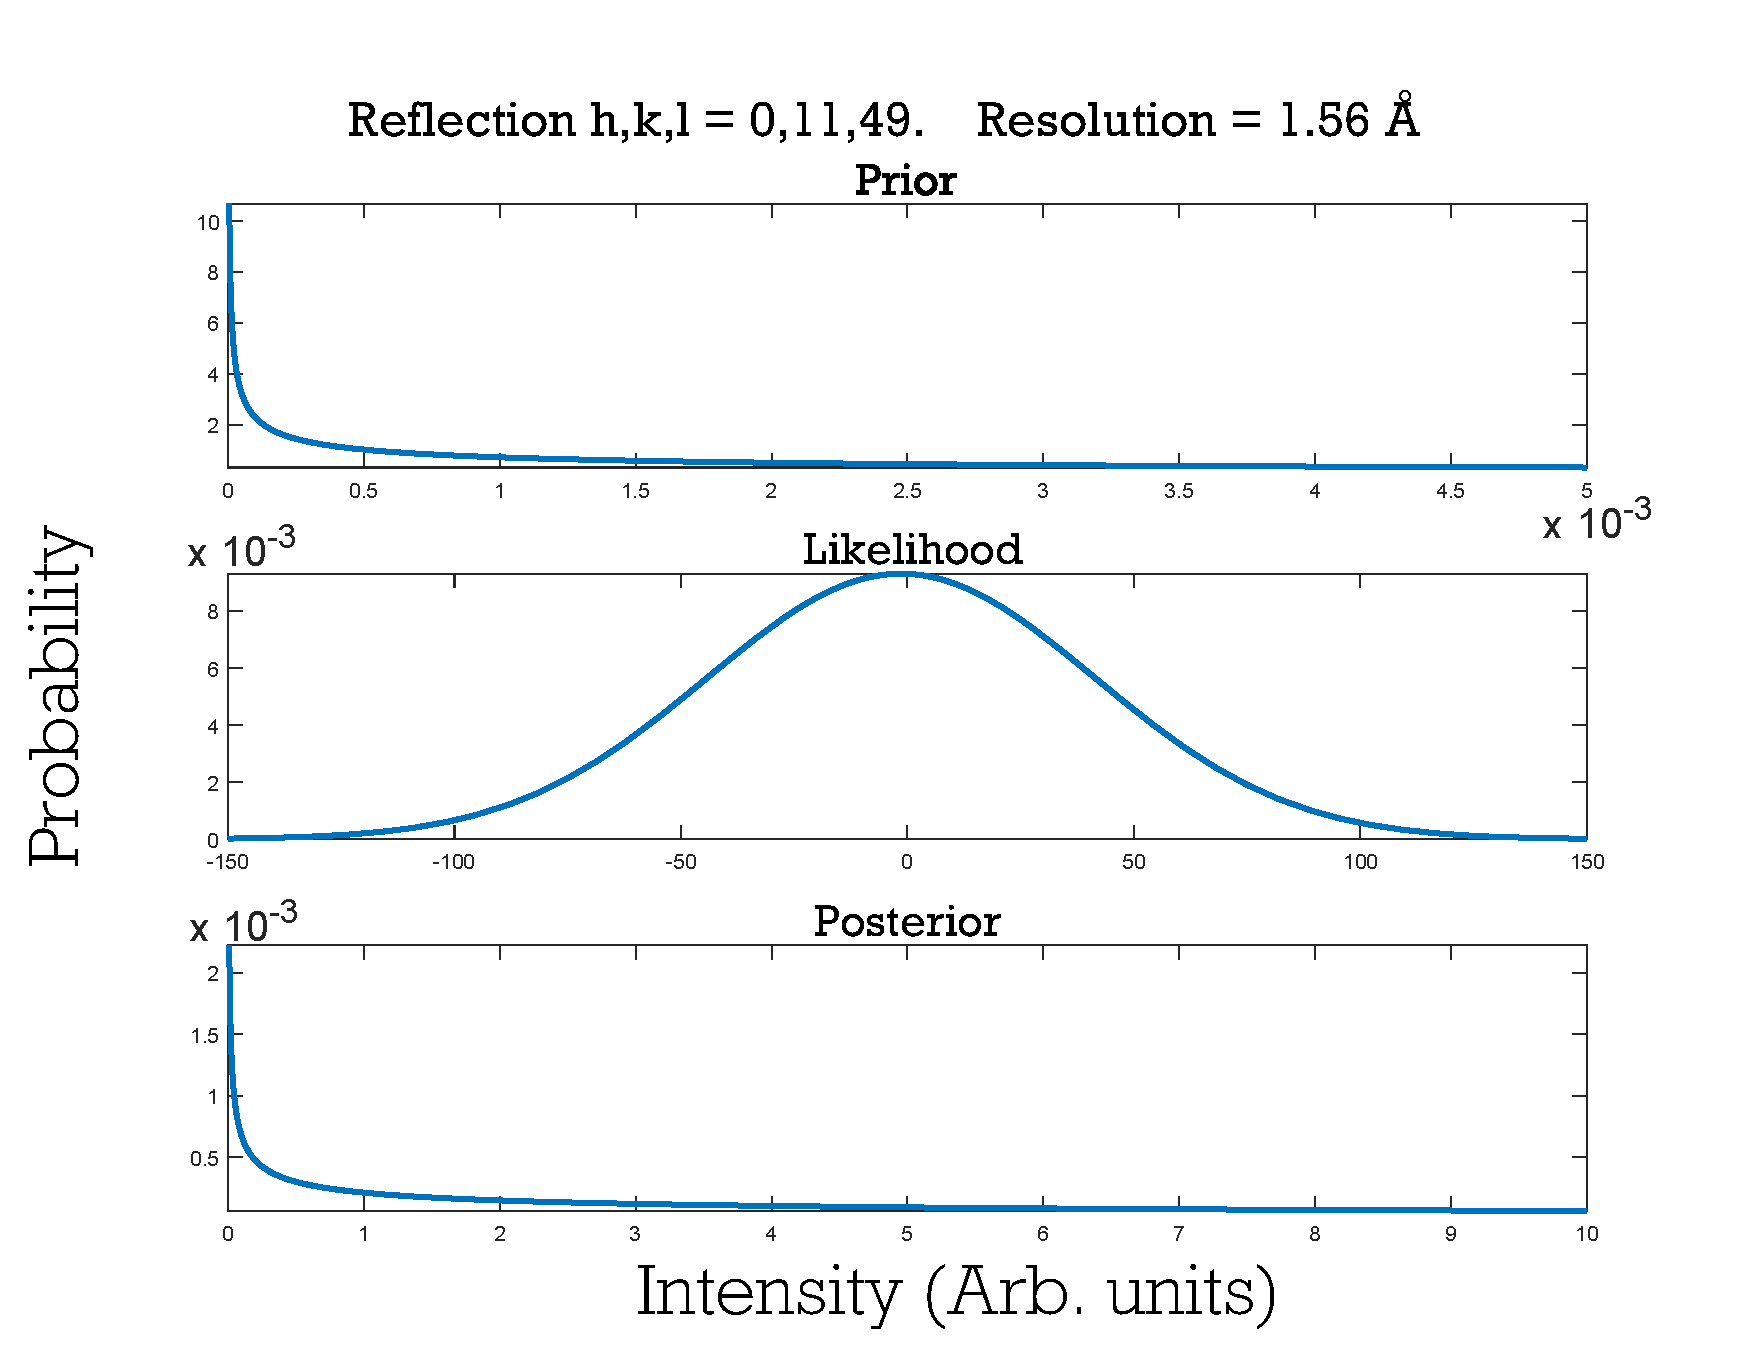
\includegraphics[width=0.9\textwidth]{figures/zde/distributions_0,11,49.pdf}
                \caption{}
                \label{fig:Weak negative reflection intensity - Extrapolation method}
        \end{subfigure}
				\\
        \begin{subfigure}[b]{0.94\textwidth}
                \centering
                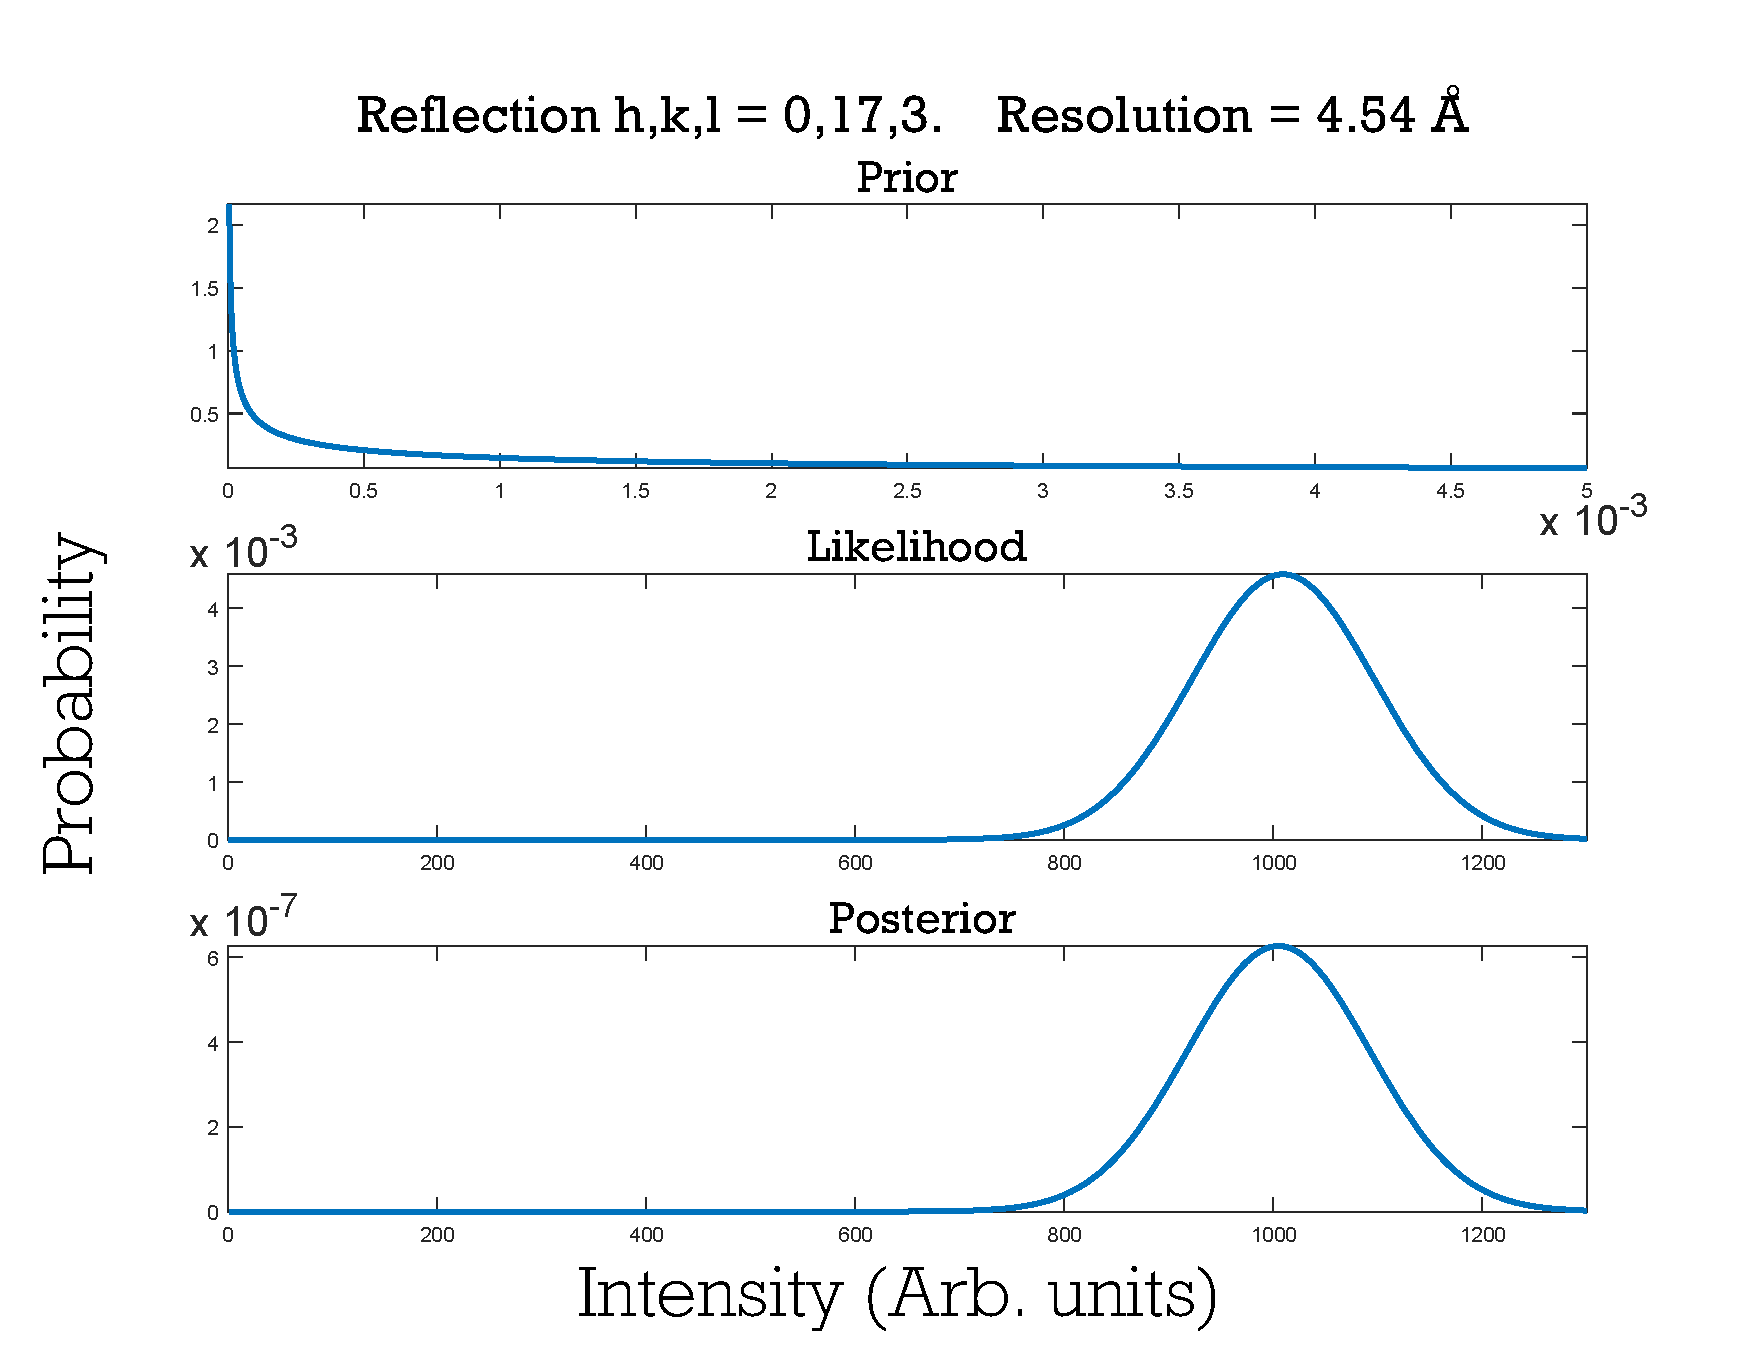
\includegraphics[width=0.9\textwidth]{figures/zde/distributions_0,17,3.pdf}
                \caption{}
                \label{fig:Strong positive reflection intensity - Extrapolation method}
        \end{subfigure}
        \caption[Prior, likelihood and (unnormalised) posterior distributions for two centric reflections.]{Prior, likelihood and (unnormalised) posterior distributions for two centric reflections.
		(a) Reflection 0,11,49. The observed intensity is negative, $I_{obs} =$ -1.4, with a relatively large standard deviation ($\sigma_{obs} =$ 42.9) in comparison.
		The posterior distribution resembles the prior distribution which is a consequence of the fact that the reflection intensity is weak.
		The resulting zero-dose value calculated as the expected value from the posterior distribution is 19.35.
		(b) Reflection 0,17,3. $I_{obs} =$ 1009.33 and $\sigma_{obs} =$ 86.99).
		This reflection is very strong ($I_{obs}/\sigma_{obs}  =$ 11.60), hence the posterior distribution resembles the likelihood distribution.
		The calculated zero-dose value is 1005.02.}
        \label{fig:Probabilistic distributions - Extrapolation method}
\end{figure}

Figure~\ref{fig:Before and after extrapolation results - Extrapolation method}  shows the intensities of all 5000 reflections before and after the extrapolation.
The overall take away message is that there is a general increase in the intensity values after performing the extrapolation.
This is expected if the true zero-dose intensity values were obtained, because the overall relative intensity decreased during the experiment (Table~\ref{tab:Average DWD and Relative Intensity}).

The red and blue solid lines in Figure~\ref{fig:Before and after extrapolation results - Extrapolation method} represent the spherically averaged intensity observations in the resolution shells before and after the extrapolation respectively.
The relative increase in the extrapolated intensities is higher on average for higher resolution reflections as evidenced by the increase in the gap between the red and blue solid lines with increasing resolution.
This is expected because the intensity of higher resolution reflections are known to decay more quickly than low resolution reflections.

There are some reflection observations that have abnormally high extrapolated intensity values.
These act to highly skew the spherically averaged mean intensity of resolution shells, as can be seen by the blue line sharply increasing for the first and last resolution shells.
These high intensity values are not a result of the regression based extrapolation because the averaged zero-dose intensities after the regression analysis do not exhibit this feature (Figure~\ref{fig:Zero-dose mean intensity in resolution shells - Extrapolation method}).
Therefore these are the result of the probabilistic extrapolation and is most likely due to applying $f(r) \approx s(D_{obs})$ to a reflection intensity where the reflection does not behave like the ``average'' reflection in the resolution shell.
These outliers could simply be rejected using suitable outlier criteria.
An obvious choice would be to reject observations where the intensity is above a given threshold.
A more sophisticated outlier rejection method using Wilson statistics could be implemented \cite{read1999detecting}.
\begin{figure}
	\centering
	\begin{subfigure}[b]{0.95\textwidth}
		\centering
		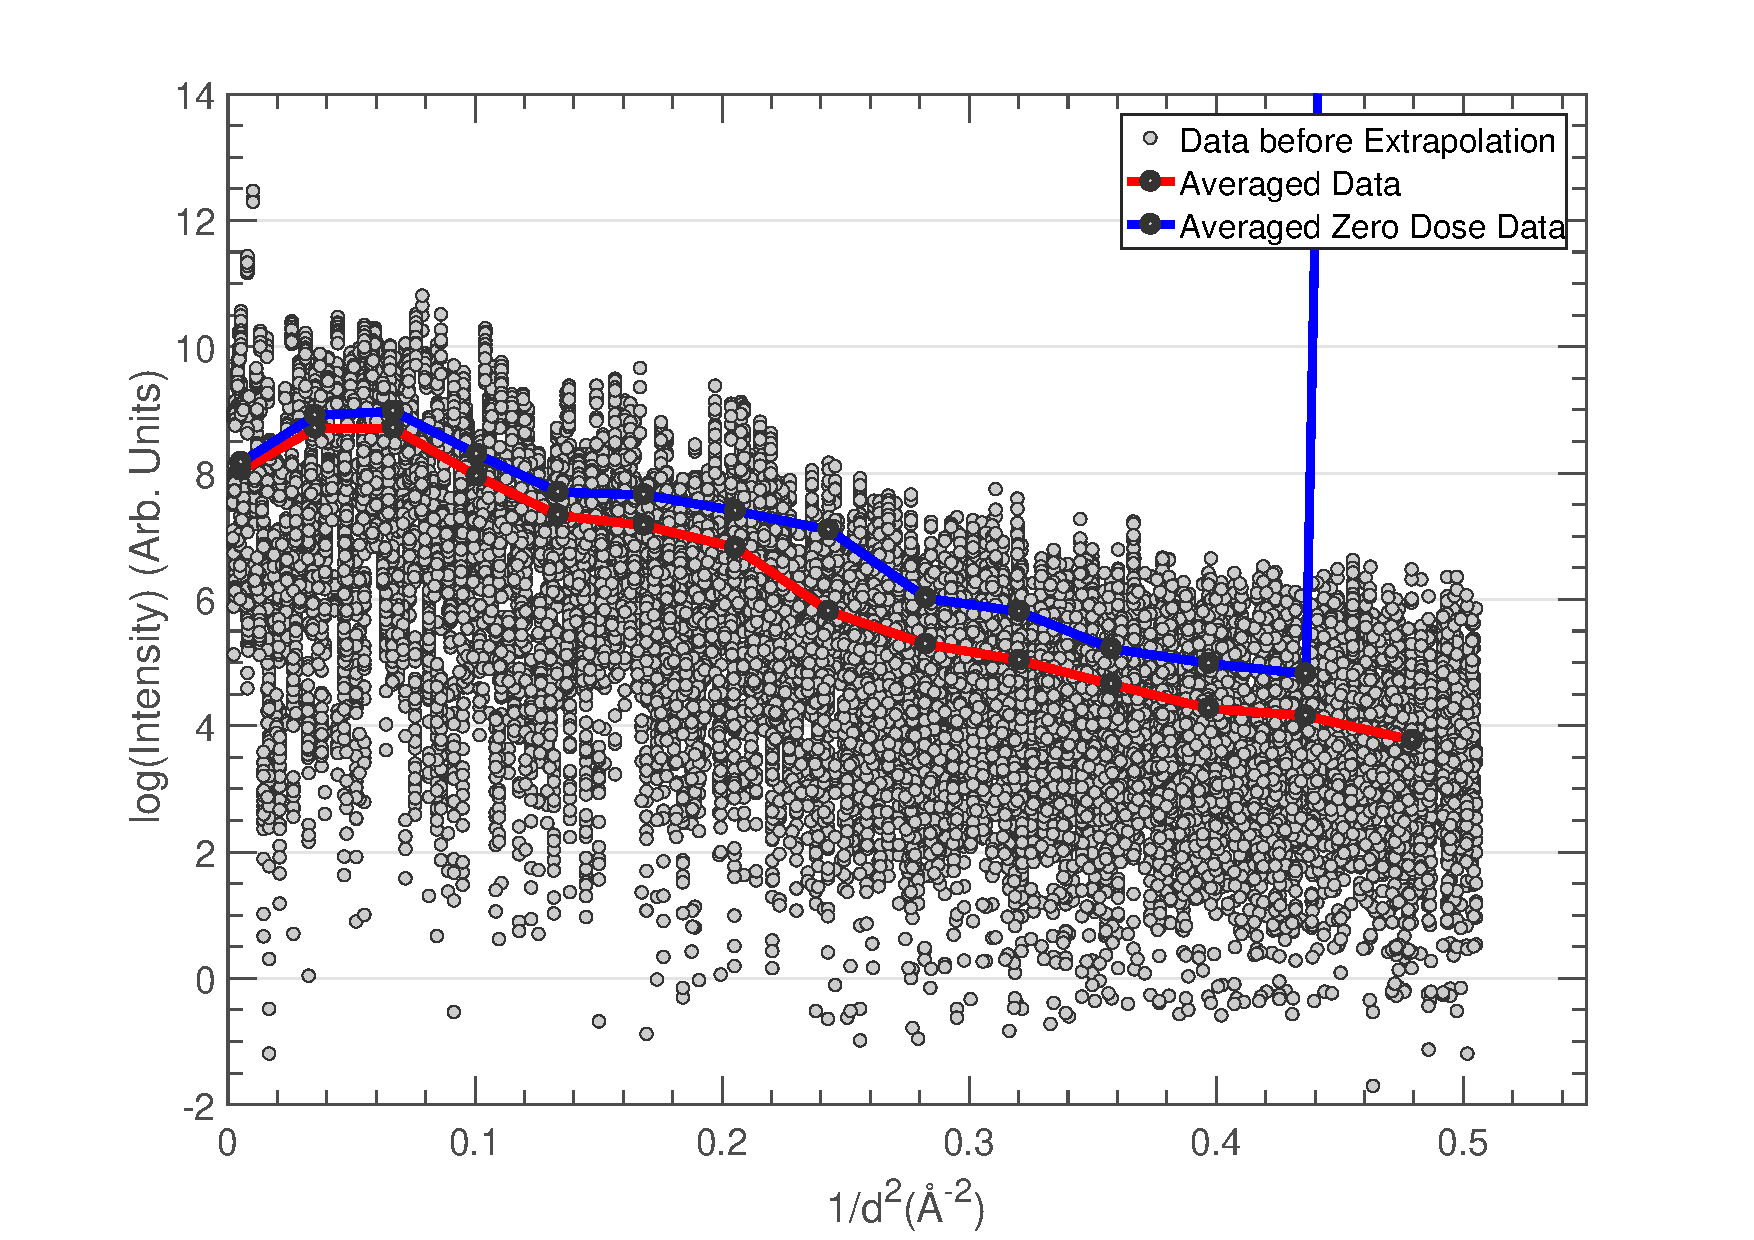
\includegraphics[width=\textwidth]{figures/zde/IntensityCurve_BeforeExtrapolation.pdf}
		\caption{}
		\label{fig:Before extrapolation all observations - Extrapolation method}
	\end{subfigure}
	\\
	\begin{subfigure}[b]{0.95\textwidth}
		\centering
		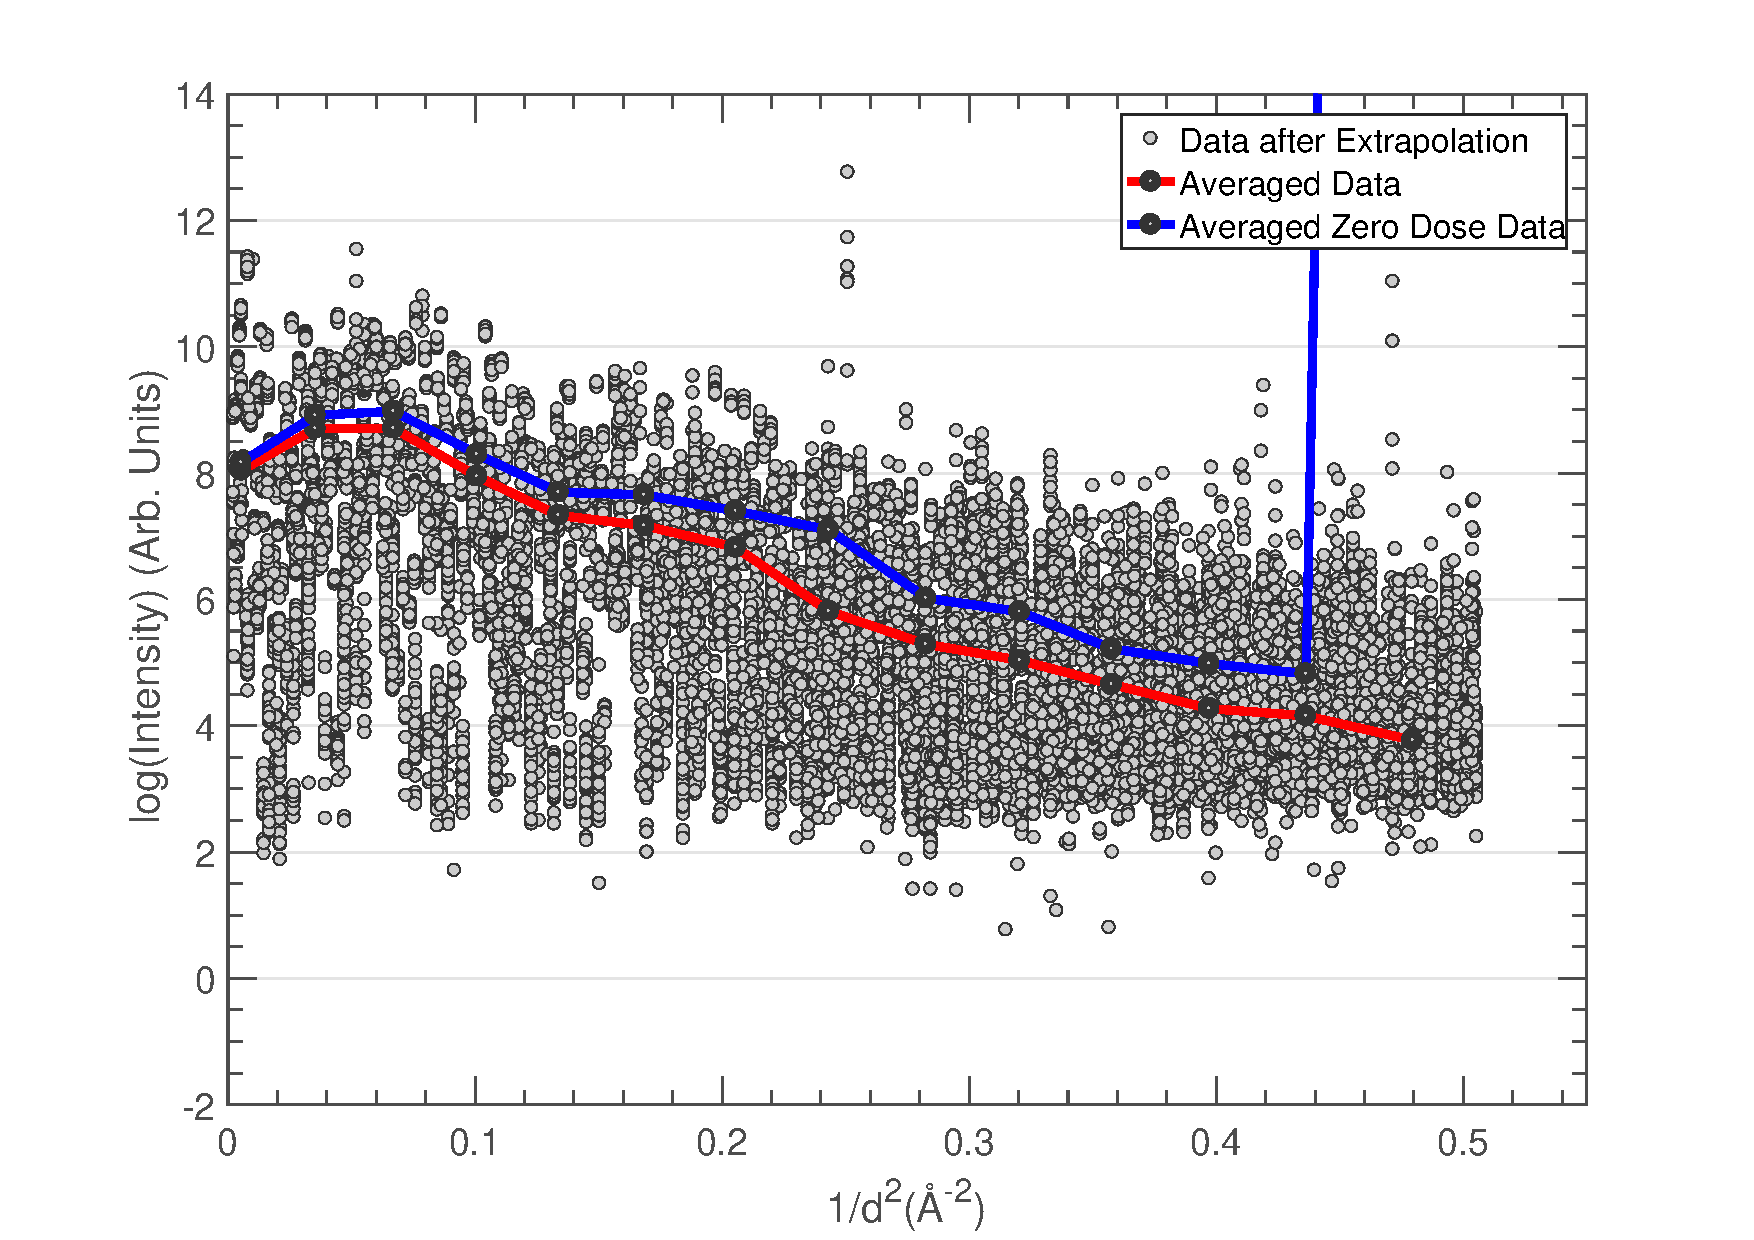
\includegraphics[width=\textwidth]{figures/zde/IntensityCurve_AfterExtrapolation.pdf}
		\caption{}
		\label{fig:After extrapolation all observations - Extrapolation method}
	\end{subfigure}
	\caption[Reflection intensities of 5000 reflections before and after zero-dose extrapolation.]{Reflection intensities of 5000 reflections before and after zero-dose extrapolation.
	The points on the red and blue solid lines represent the mean intensity of the resolution shells before and after the extrapolation respectively.
	As expected, there is a general increase in the reflection intensities after extrapolation.}
	\label{fig:Before and after extrapolation results - Extrapolation method}
\end{figure}
